\subsubsection*{Experimentación}
\textbf{Test RedFull}
En este primer experimento analizamos la influencia en los resultados de las diferentes variables de experimentación que manejamos utilizando tanto el método KNN como el KNN + PCA. Las mismas son la cantidad de vecinos considerados por KNN (k), y la cantidad de componentes principales de la imagen transformada ($\alpha$).


En este caso podemos observar una relación entre las dos variables, a medida que el $\alpha$ aumenta vemos como también lo hace nuestro accuracy.

Como expresamos anteriormente (COMPLETRAR), debido al funcionamiento de PCA esperábamos que a mayor $\alpha$, mejores sean nuestros resultados (todas nuestras métricas en general) y por lo tanto nuestro accuracy también.

Pero a su vez tambien vimos que un $\alpha$ muy elevado  nos elevaría el tiempo de ejecución y a su vez en este gráfico vemos como las diferencias entre accuracy son cada vez menores (por ejemplo entre $\alpha$ = 10 y $\alpha$ = 50).

En base a los resultados obtenidos concluimos que un valor de $\alpha$ cercano a 10 nos daría un buen balance entre relativamente la cantidad de componentes principales y la efectividad (se sacrifica algo de efectividad pero se gana en trabajar con imágenes más chicas)

\begin{figure}[H]
	\centering	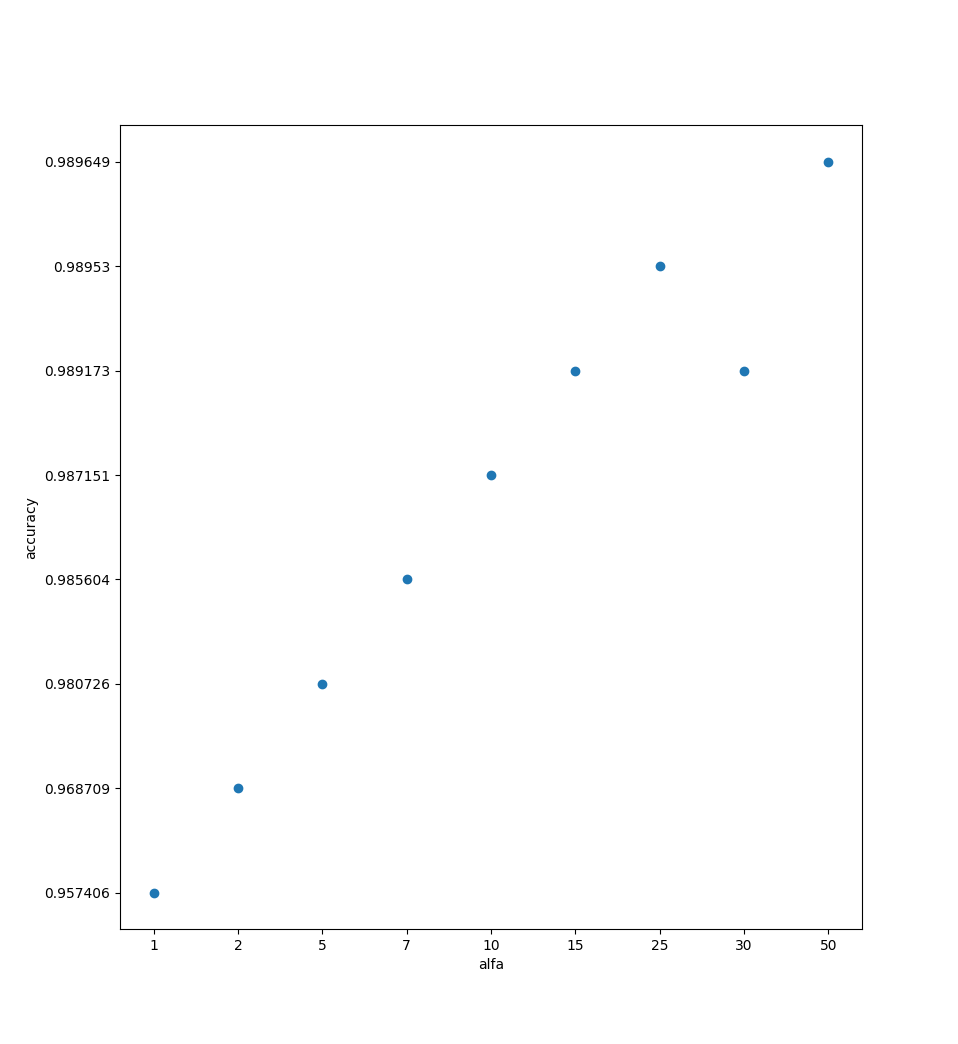
\includegraphics[width=0.9\textwidth]{img/alfa_pca_accu.png}
	\caption{Accuracy vs $\alpha$ con PCA + KNN}
	\label{fig:Accuracy vs Alpha con KNN + PCA}
\end{figure}

\begin{figure}[H]
	\centering	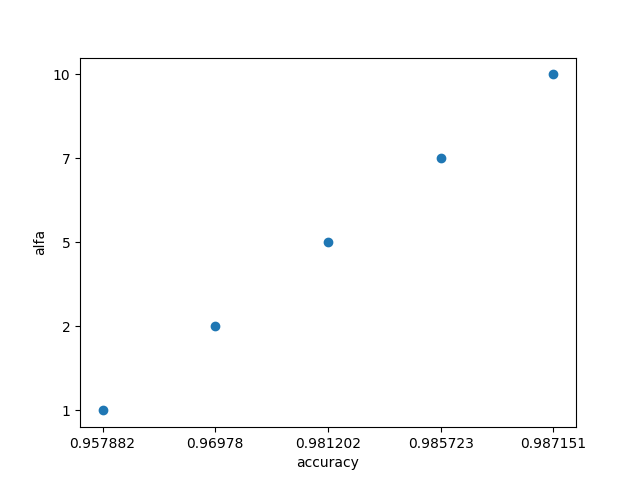
\includegraphics[width=0.9\textwidth]{img/big_alfa_pca_accu.png}
	\caption{BIG Accuracy vs $\alpha$ con PCA + KNN}
	\label{fig: BIG Accuracy vs Alpha con KNN + PCA}
\end{figure}



Tal como esperabamos vemos que a medida que el $\alpha$ aumenta (es decir, cuantas más componentes principales tengamos), el tiempo de ejecución también lo hace.

Luego, en línea con los resultados de los gráficos anteriores (Accuracy vs $\alpha$) podemos volver a afirmar que un $\alpha$ cercano a 10 sería un buen balance. En este gráfico notamos si tomaramos alfa = 30, tardaría aproximadamente el triple y no obtendríamos una mejora sustancial en el accuracy.
\begin{figure}[H]
	\centering	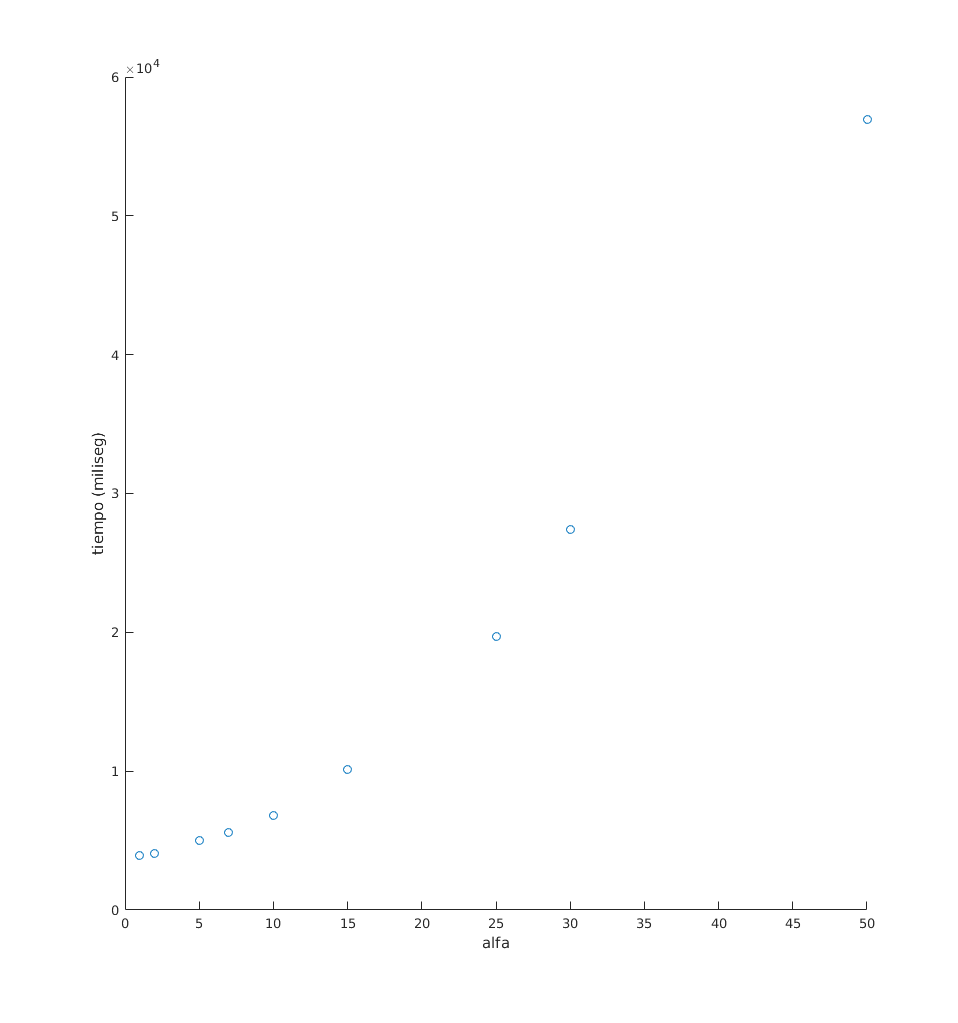
\includegraphics[width=0.9\textwidth]{img/alfa_pca_tiempo.png}
	\caption{Tiempo vs $\alpha$ con PCA + KNN}
	\label{fig:Tiempo vs Alpha con PCA + KNN}
\end{figure}

\begin{figure}[H]
	\centering	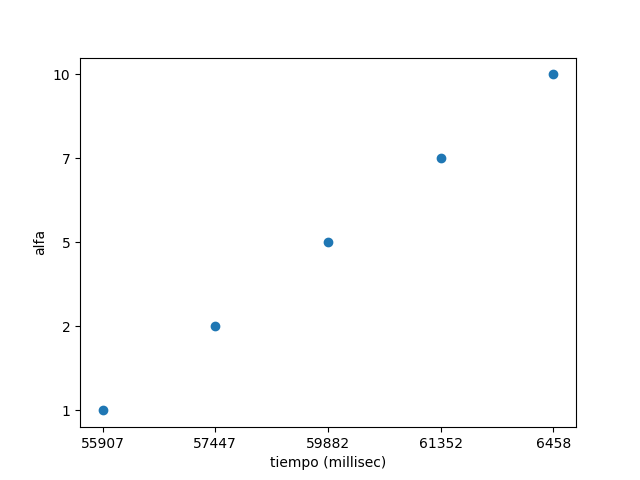
\includegraphics[width=0.9\textwidth]{img/big_alfa_pca_tiempo.png}
	\caption{Big Tiempo vs $\alpha$ con PCA + KNN}
	\label{fig:Big Tiempo vs Alpha con PCA + KNN}
\end{figure}





\begin{figure}[H]
	\centering	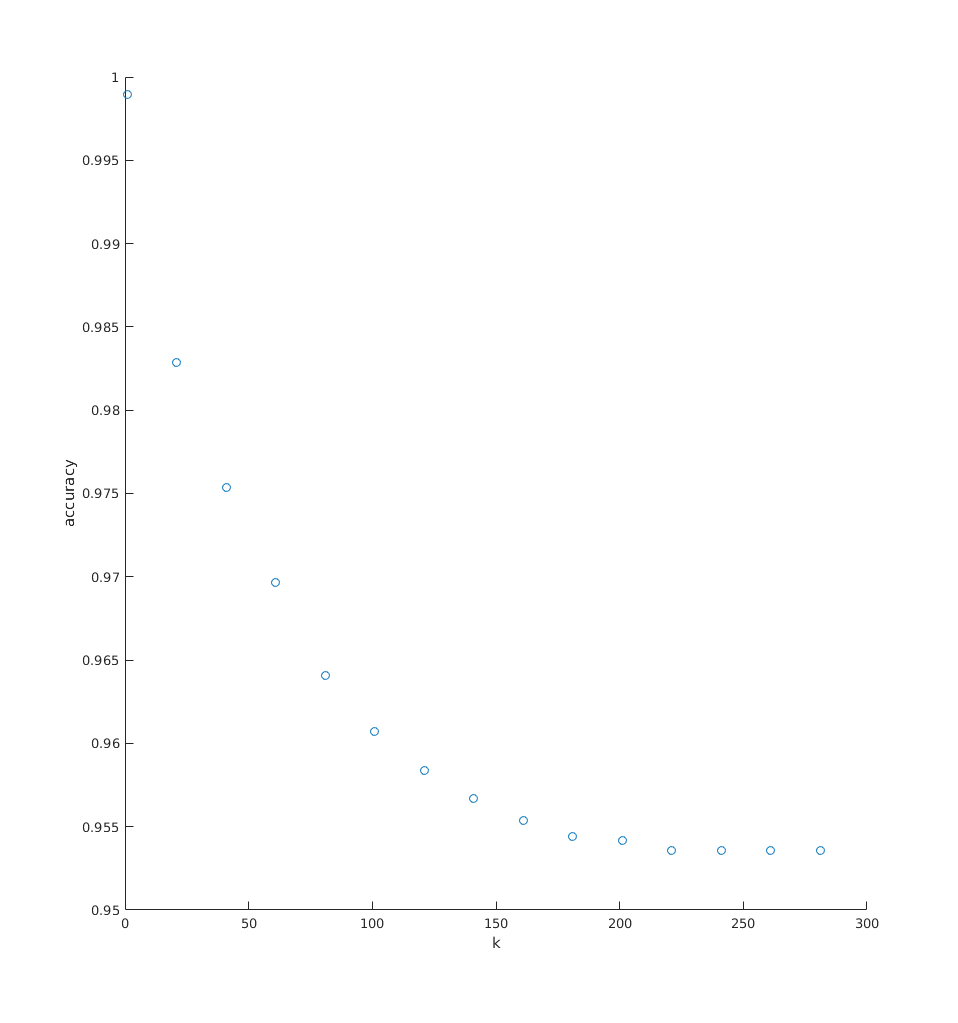
\includegraphics[width=0.9\textwidth]{img/k_knn_accu.png}
	\caption{Accuracy va K con KNN}
	\label{fig:Accuracy vs K con KNN}
\end{figure}
\begin{figure}[H]
	\centering	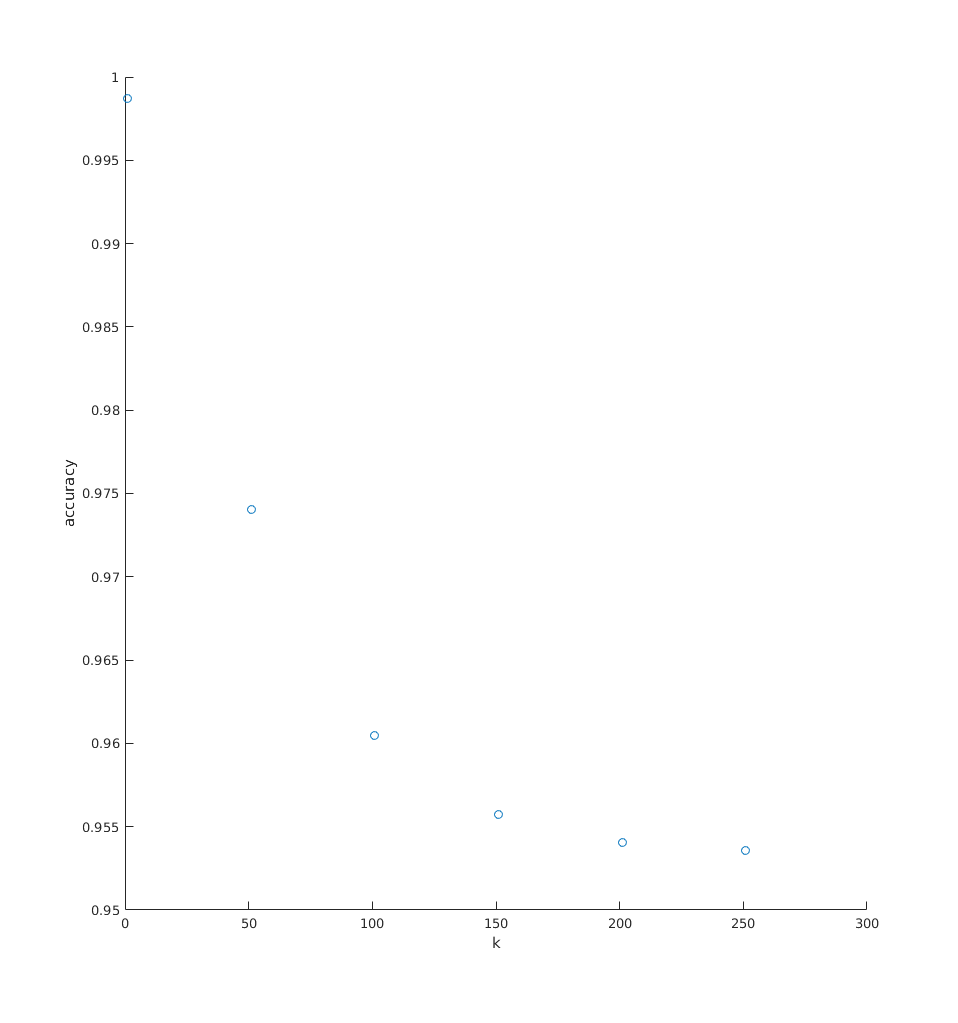
\includegraphics[width=0.9\textwidth]{img/big_k_knn_accu.png}
	\caption{Big Accuracy vs K con KNN}
	\label{fig:Big Accuracy vs K con KNN}
\end{figure}






\begin{figure}[H]
	\centering	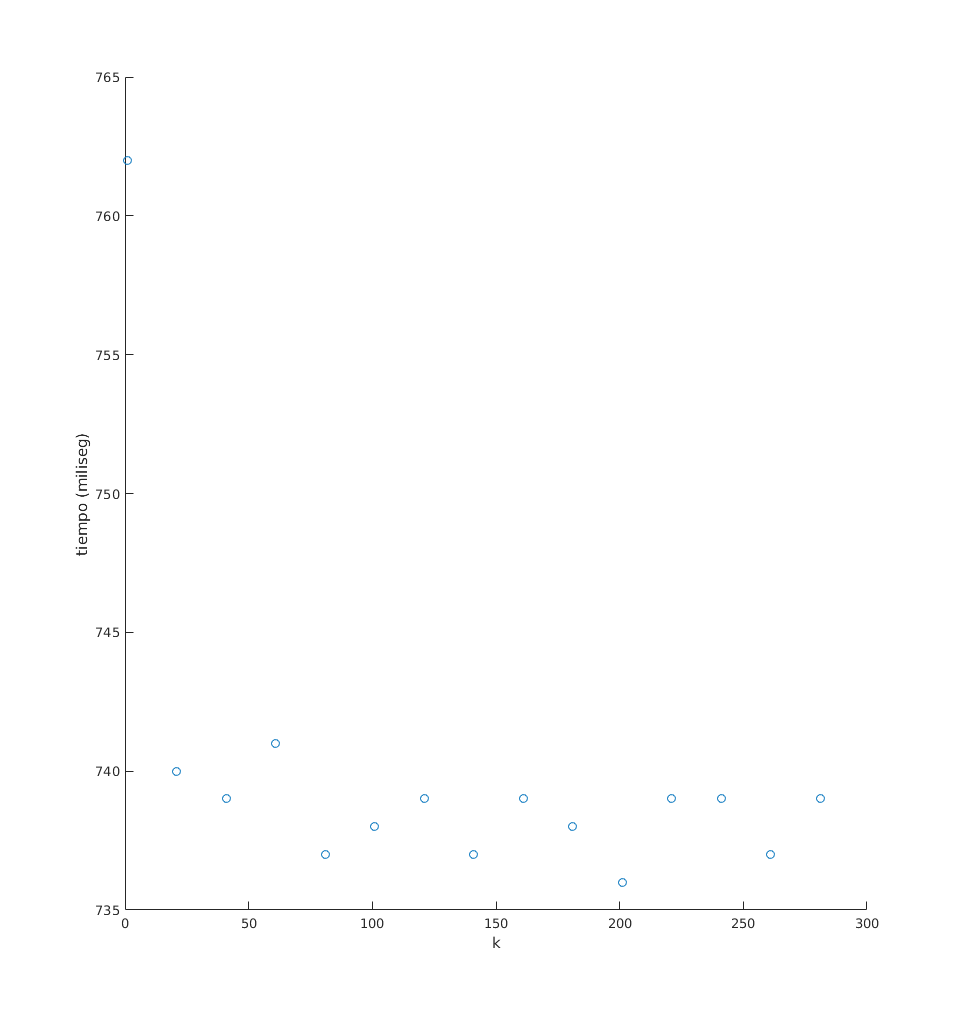
\includegraphics[width=0.9\textwidth]{img/k_knn_tiempo.png}
	\caption{Tiempo vs K con KNN}
	\label{fig:K vs Tiempo con KNN}
\end{figure}
\begin{figure}[H]
	\centering	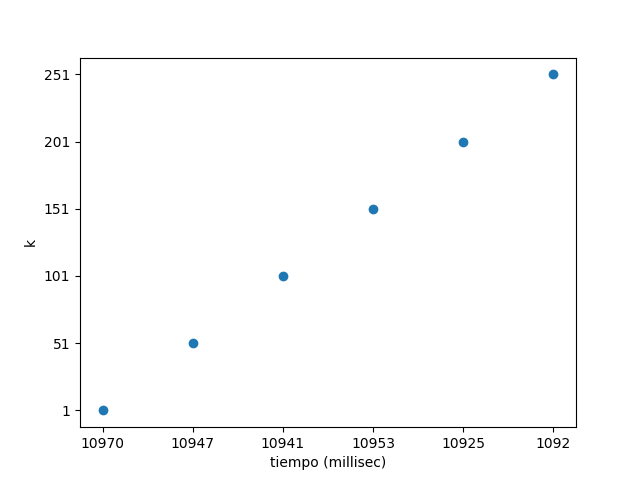
\includegraphics[width=0.9\textwidth]{img/big_k_knn_tiempo.png}
	\caption{Big Tiempo vs K con KNN}
	\label{fig:Big K vs Tiempo con KNN}
\end{figure}





\begin{figure}[H]
	\centering	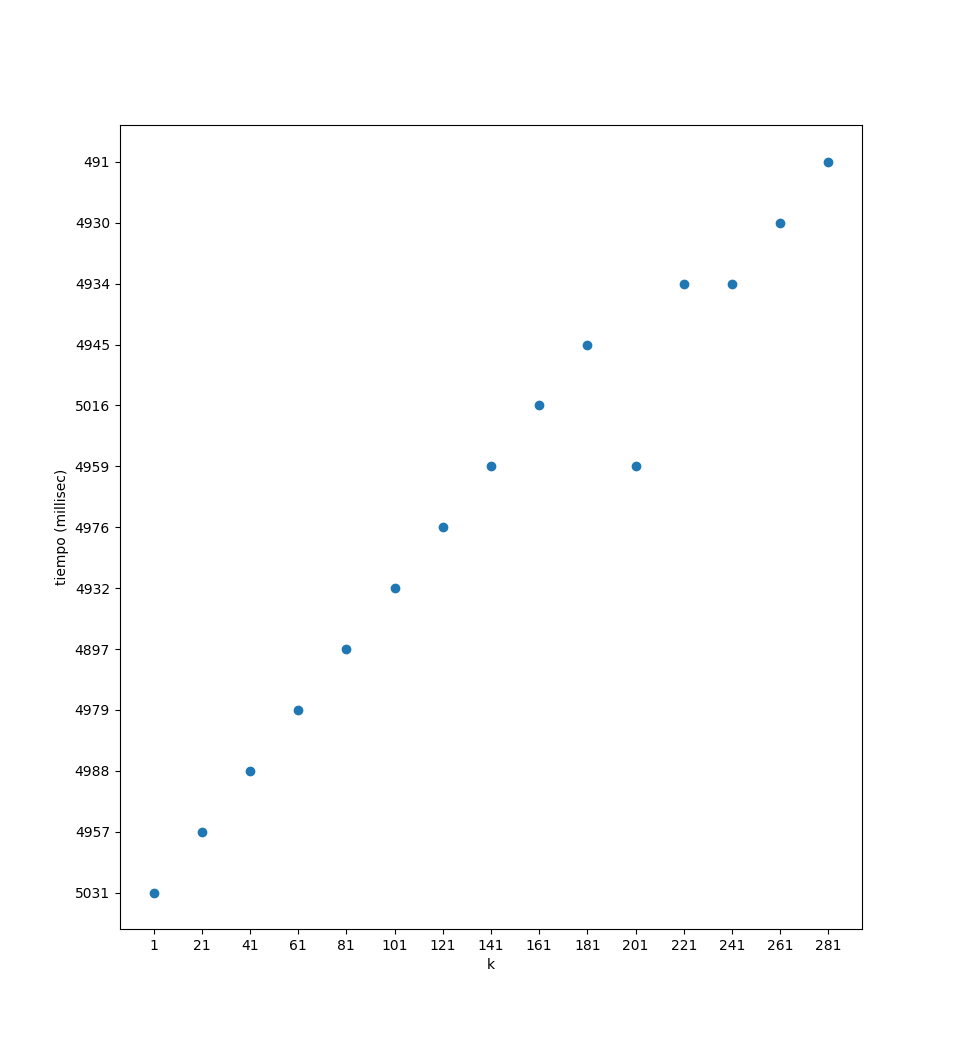
\includegraphics[width=0.9\textwidth]{img/k_pca_tiempo.png}
	\caption{K vs Tiempo con KNN + PCA}
	\label{fig:K vs Tiempo con KNN + PCA}
\end{figure}
\begin{figure}[H]
	\centering	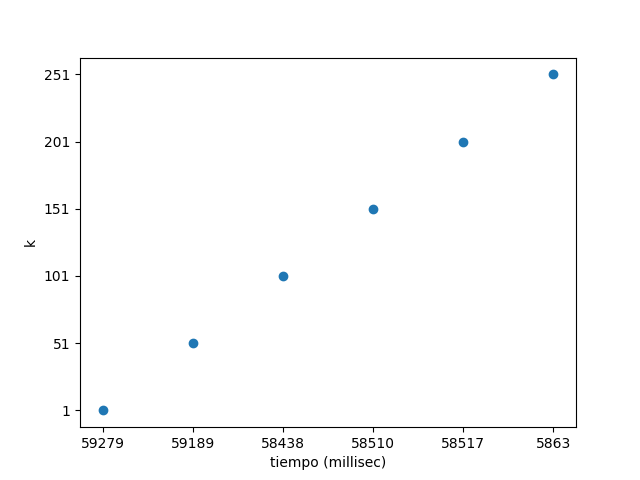
\includegraphics[width=0.9\textwidth]{img/big_k_pca_tiempo.png}
	\caption{Big Tiempo vs K con KNN + PCA}
	\label{fig:Big K vs Tiempo con KNN + PCA}
\end{figure}



Y por último en este caso vemos una estrecha relación entre cuantos vecinos cercanos tomamos y el accuracy.

Esto se debe a que al tomar más vecinos cercanos nos exponemos a un error mayor debido a que le estaríamos dando el mismo peso a todos esos K vecinos sin importar que tan cerca estén de la imagen testeada.

Llevando esto a un extremo podríamos tomar K = "Tamaño de matriz de entrenamiento" y cualquiera de las clases tendría el mismo peso con lo que perdería sentido este método.

Por otro lado tampoco es conveniente tener un K demasiado chico. Por ejemplo, si tomaramos K = 1 asociaríamos la imagen a testear con la que esté a menor distancia, que debido a alguna diferencia la forma en que fue tomada la imagen puede no pertenecer a la clase de la imagen testeada.

Es llegamos a la conclusión de que utilizando un valor de K cercano a 10 obtenemos la mejor relación (dentro de nuestro set de tests).
Por un lado evitamos el problema que ocurre cuando K es demasiado grande y por otro, tomamos una cantidad de imágenes cercanas suficiente como para minimizar el impacto de algún outsider.
\begin{figure}[H]
	\centering
	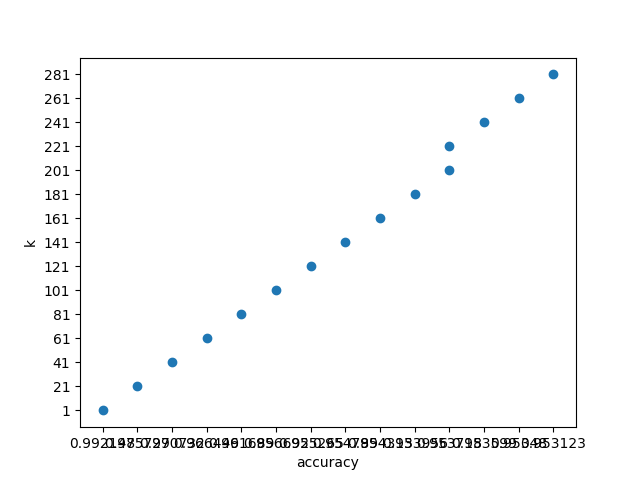
\includegraphics[width=0.9\textwidth]{img/k_pca_accu.png}
	\caption{Accuracy vs K con KNN + PCA}
	\label{fig:K vs Accuracy con KNN + PCA}
\end{figure}


Conclusión:
Luego de observar estos gráficos llegamos a algunas conclusiones.
En cuanto al tiempo, por un lado, la cantidad de vecinos cercanos que tomemos no afecta significativamente el tiempo, pero lo que sí lo afecta es el $\alpha$ de PCA.
A qué se debe esto? Teniendo en cuenta el funcionamiento de nuestro algoritmo, entendemos que esto se debe a que una gran parte del tiempo de procesamiento de PCA se consume en el método de la potencia (que se realiza $\alpha$ veces) y en la transformación de los autovectores calculados en los de la verdadera matriz de covarianza de la muestra, que involucran numerosos cálculos matriciales.

Sin embargo, pensamos que en una implementación real estaríamos trabajando con una única training base, y las transformaciones que llevamos a cabo en el PCA las haríamos una única vez, con lo que este costo de tiempo se pagaría solamente una vez o cuando sea necesario agregar o quitar alguna imagen, para luego realizar únicamente el reconocimiento. Usando PCA + KNN tenemos la ventaja de trabajar con imágenes de menor tamaño con el consiguiente ahorro de espacio.